\documentclass[]{book}
\usepackage{lmodern}
\usepackage{amssymb,amsmath}
\usepackage{ifxetex,ifluatex}
\usepackage{fixltx2e} % provides \textsubscript
\ifnum 0\ifxetex 1\fi\ifluatex 1\fi=0 % if pdftex
  \usepackage[T1]{fontenc}
  \usepackage[utf8]{inputenc}
\else % if luatex or xelatex
  \ifxetex
    \usepackage{mathspec}
  \else
    \usepackage{fontspec}
  \fi
  \defaultfontfeatures{Ligatures=TeX,Scale=MatchLowercase}
\fi
% use upquote if available, for straight quotes in verbatim environments
\IfFileExists{upquote.sty}{\usepackage{upquote}}{}
% use microtype if available
\IfFileExists{microtype.sty}{%
\usepackage{microtype}
\UseMicrotypeSet[protrusion]{basicmath} % disable protrusion for tt fonts
}{}
\usepackage[margin=1in]{geometry}
\usepackage{hyperref}
\hypersetup{unicode=true,
            pdftitle={Badges in Education},
            pdfauthor={Peter Baumgartner},
            pdfborder={0 0 0},
            breaklinks=true}
\urlstyle{same}  % don't use monospace font for urls
\usepackage{natbib}
\bibliographystyle{apalike}
\usepackage{color}
\usepackage{fancyvrb}
\newcommand{\VerbBar}{|}
\newcommand{\VERB}{\Verb[commandchars=\\\{\}]}
\DefineVerbatimEnvironment{Highlighting}{Verbatim}{commandchars=\\\{\}}
% Add ',fontsize=\small' for more characters per line
\usepackage{framed}
\definecolor{shadecolor}{RGB}{248,248,248}
\newenvironment{Shaded}{\begin{snugshade}}{\end{snugshade}}
\newcommand{\KeywordTok}[1]{\textcolor[rgb]{0.13,0.29,0.53}{\textbf{#1}}}
\newcommand{\DataTypeTok}[1]{\textcolor[rgb]{0.13,0.29,0.53}{#1}}
\newcommand{\DecValTok}[1]{\textcolor[rgb]{0.00,0.00,0.81}{#1}}
\newcommand{\BaseNTok}[1]{\textcolor[rgb]{0.00,0.00,0.81}{#1}}
\newcommand{\FloatTok}[1]{\textcolor[rgb]{0.00,0.00,0.81}{#1}}
\newcommand{\ConstantTok}[1]{\textcolor[rgb]{0.00,0.00,0.00}{#1}}
\newcommand{\CharTok}[1]{\textcolor[rgb]{0.31,0.60,0.02}{#1}}
\newcommand{\SpecialCharTok}[1]{\textcolor[rgb]{0.00,0.00,0.00}{#1}}
\newcommand{\StringTok}[1]{\textcolor[rgb]{0.31,0.60,0.02}{#1}}
\newcommand{\VerbatimStringTok}[1]{\textcolor[rgb]{0.31,0.60,0.02}{#1}}
\newcommand{\SpecialStringTok}[1]{\textcolor[rgb]{0.31,0.60,0.02}{#1}}
\newcommand{\ImportTok}[1]{#1}
\newcommand{\CommentTok}[1]{\textcolor[rgb]{0.56,0.35,0.01}{\textit{#1}}}
\newcommand{\DocumentationTok}[1]{\textcolor[rgb]{0.56,0.35,0.01}{\textbf{\textit{#1}}}}
\newcommand{\AnnotationTok}[1]{\textcolor[rgb]{0.56,0.35,0.01}{\textbf{\textit{#1}}}}
\newcommand{\CommentVarTok}[1]{\textcolor[rgb]{0.56,0.35,0.01}{\textbf{\textit{#1}}}}
\newcommand{\OtherTok}[1]{\textcolor[rgb]{0.56,0.35,0.01}{#1}}
\newcommand{\FunctionTok}[1]{\textcolor[rgb]{0.00,0.00,0.00}{#1}}
\newcommand{\VariableTok}[1]{\textcolor[rgb]{0.00,0.00,0.00}{#1}}
\newcommand{\ControlFlowTok}[1]{\textcolor[rgb]{0.13,0.29,0.53}{\textbf{#1}}}
\newcommand{\OperatorTok}[1]{\textcolor[rgb]{0.81,0.36,0.00}{\textbf{#1}}}
\newcommand{\BuiltInTok}[1]{#1}
\newcommand{\ExtensionTok}[1]{#1}
\newcommand{\PreprocessorTok}[1]{\textcolor[rgb]{0.56,0.35,0.01}{\textit{#1}}}
\newcommand{\AttributeTok}[1]{\textcolor[rgb]{0.77,0.63,0.00}{#1}}
\newcommand{\RegionMarkerTok}[1]{#1}
\newcommand{\InformationTok}[1]{\textcolor[rgb]{0.56,0.35,0.01}{\textbf{\textit{#1}}}}
\newcommand{\WarningTok}[1]{\textcolor[rgb]{0.56,0.35,0.01}{\textbf{\textit{#1}}}}
\newcommand{\AlertTok}[1]{\textcolor[rgb]{0.94,0.16,0.16}{#1}}
\newcommand{\ErrorTok}[1]{\textcolor[rgb]{0.64,0.00,0.00}{\textbf{#1}}}
\newcommand{\NormalTok}[1]{#1}
\usepackage{longtable,booktabs}
\usepackage{graphicx,grffile}
\makeatletter
\def\maxwidth{\ifdim\Gin@nat@width>\linewidth\linewidth\else\Gin@nat@width\fi}
\def\maxheight{\ifdim\Gin@nat@height>\textheight\textheight\else\Gin@nat@height\fi}
\makeatother
% Scale images if necessary, so that they will not overflow the page
% margins by default, and it is still possible to overwrite the defaults
% using explicit options in \includegraphics[width, height, ...]{}
\setkeys{Gin}{width=\maxwidth,height=\maxheight,keepaspectratio}
\IfFileExists{parskip.sty}{%
\usepackage{parskip}
}{% else
\setlength{\parindent}{0pt}
\setlength{\parskip}{6pt plus 2pt minus 1pt}
}
\setlength{\emergencystretch}{3em}  % prevent overfull lines
\providecommand{\tightlist}{%
  \setlength{\itemsep}{0pt}\setlength{\parskip}{0pt}}
\setcounter{secnumdepth}{5}
% Redefines (sub)paragraphs to behave more like sections
\ifx\paragraph\undefined\else
\let\oldparagraph\paragraph
\renewcommand{\paragraph}[1]{\oldparagraph{#1}\mbox{}}
\fi
\ifx\subparagraph\undefined\else
\let\oldsubparagraph\subparagraph
\renewcommand{\subparagraph}[1]{\oldsubparagraph{#1}\mbox{}}
\fi

%%% Use protect on footnotes to avoid problems with footnotes in titles
\let\rmarkdownfootnote\footnote%
\def\footnote{\protect\rmarkdownfootnote}

%%% Change title format to be more compact
\usepackage{titling}

% Create subtitle command for use in maketitle
\newcommand{\subtitle}[1]{
  \posttitle{
    \begin{center}\large#1\end{center}
    }
}

\setlength{\droptitle}{-2em}
  \title{Badges in Education}
  \pretitle{\vspace{\droptitle}\centering\huge}
  \posttitle{\par}
  \author{Peter Baumgartner}
  \preauthor{\centering\large\emph}
  \postauthor{\par}
  \predate{\centering\large\emph}
  \postdate{\par}
  \date{2018-05-23}

\usepackage{booktabs}
\usepackage{booktabs}
\usepackage{longtable}
\usepackage{array}
\usepackage{multirow}
\usepackage[table]{xcolor}
\usepackage{wrapfig}
\usepackage{float}
\usepackage{colortbl}
\usepackage{pdflscape}
\usepackage{tabu}
\usepackage{threeparttable}
\usepackage{threeparttablex}
\usepackage[normalem]{ulem}
\usepackage{makecell}

\usepackage{amsthm}
\newtheorem{theorem}{Theorem}[chapter]
\newtheorem{lemma}{Lemma}[chapter]
\theoremstyle{definition}
\newtheorem{definition}{Definition}[chapter]
\newtheorem{corollary}{Corollary}[chapter]
\newtheorem{proposition}{Proposition}[chapter]
\theoremstyle{definition}
\newtheorem{example}{Example}[chapter]
\theoremstyle{definition}
\newtheorem{exercise}{Exercise}[chapter]
\theoremstyle{remark}
\newtheorem*{remark}{Remark}
\newtheorem*{solution}{Solution}
\begin{document}
\maketitle

{
\setcounter{tocdepth}{1}
\tableofcontents
}
\chapter{Preface}\label{preface}

Still to write

\chapter{Introduction}\label{intro}

Still to write

\chapter{Badges in StackOverflow}\label{badges-in-stackoverflow}

\section{Categorization of Badges}\label{categorization-of-badges}

I need to download all types of badges with their description and for
further investigation to categorize them.

\subsection{Badges for different
activities}\label{badges-for-different-activities}

The badges are grouped according to the necessary activities to get
them. The different types of badges can be seen on
\href{https://stackoverflow.com/help/badges}{help page for badges}:

\begin{enumerate}
\def\labelenumi{\arabic{enumi})}
\tightlist
\item
  Question badges
\item
  Answer badges
\item
  Partication badges
\item
  Moderation badges
\item
  Other badges
\item
  Documentation badges
\end{enumerate}

\subsection{Badges from different
sources}\label{badges-from-different-sources}

Another differentiation is the point of origin the badges come from.
Even though all badges are generated automatically by the system, there
are two principal sources to get them. There are two different entities
responsible for awarding badges.

\begin{enumerate}
\def\labelenumi{\arabic{enumi}.}
\tightlist
\item
  There are badges you can get by just doing a certain action once or a
  needed number of times.
\item
  And there are badges you get only after some community action.
\end{enumerate}

I call the first type \texttt{user} and the second type
\texttt{community} badges.

\textbf{Examples for \texttt{user} badges:}

Name: ``Civic Duty'' (Vote 300 times). Name: ``Enthusiast'' (Visit the
site each day for 30 consecutive day)

Some of the \texttt{user} badges are only available after some threshold
value is reached and a certain privileges is granted. For instance
voting up needs 15 and voting down 125 reputation points.

\textbf{Examples for \texttt{community} badges:}

Name: ``Favorite Question'' (Question favored by 25 users) Name:
``Popular Question'' (Question with 1000 views).

There are also badges tied with certain events, like moderator election,
working with the beta version, meeting employees at an event etc. Mostly
these badges are in my categorization \texttt{user} badges, but you
cannot get them at any time, even if you would have the required
privileges.

The badge system of Stack Overflow is a dynamic system. When the website
was launched (Spetember 15, 2008) it did not start with all 91 badges
which are listed today (May 21, 2018). Some of the badges were added
during the history of the website but other are not awared anymore. Some
of those badges which are not functional anymore are retired badges
(e.g. ``Analytical'', for visiting all sections of the FAQ). This means
you will still see some veteran users with these badges. Other badges
(all three documentation badges for instance) are withdrawn, e.g.~they
were even deleted from those user accounts they were awarded earlier. I
call these two groups of badges \texttt{event} and \texttt{dead} badges.

To sum up there are 4 point of origins for badges:

\begin{enumerate}
\def\labelenumi{\arabic{enumi})}
\tightlist
\item
  Badges from user action = \texttt{user} badges
\item
  Badges from community action = \texttt{community} badges
\item
  Badges from some action during a specified occurence = \texttt{event}
  badges
\item
  Badges where the point of origin is not interesting anymore as they
  are now non-funtional = \texttt{dead} badges
\end{enumerate}

\begin{landscape}\rowcolors{2}{white}{gray!6}

\begin{longtable}[t]{lr>{\raggedright\arraybackslash}p{2cm}rlll>{\raggedright\arraybackslash}p{10cm}}
\caption{\label{tab:display-badges-table-landscape}Badges in Stack Overflow}\\
\hiderowcolors
\toprule
  & ID & Name & Count & Rank & Activity & Origin & Description\\
\midrule
\endfirsthead
\caption[]{\label{tab:display-badges-table-landscape}Badges in Stack Overflow \textit{(continued)}}\\
\toprule
  & ID & Name & Count & Rank & Activity & Origin & Description\\
\midrule
\endhead
\
\endfoot
\bottomrule
\endlastfoot
\showrowcolors
1 & 222 & Altruist & 8158 & bronze & Question & User & First bounty you manually award on another person\&\#39;s question\\
2 & 1306 & Analytical & 43743 & bronze & Other & Dead & Visited every section of the FAQ (retired)\\
3 & 260 & Announcer & 131289 & bronze & Other & Community & Share a link to a question later visited by 25 unique IP addresses\\
4 & 1286 & Archaeologist & 1883 & silver & Moderation & User & Edit 100 posts that were inactive for 6 months\\
5 & 9 & Autobiographer & 799567 & bronze & Participation & User & Complete \&quot;About Me\&quot; section of user profile\\
\addlinespace
6 & 221 & Benefactor & 38879 & bronze & Question & User & First bounty you manually award on your own question\\
7 & 30 & Beta & 2510 & silver & Participation & Event & Voted 10 times, added 3 posts score \&gt; 0, and visited the site on 3 separate days during the private beta\\
8 & 261 & Booster & 3234 & silver & Other & Community & Share a link to a question later visited by 300 unique IP addresses\\
9 & 1973 & Caucus & 573681 & bronze & Participation & Event & Visit an <a href="https://stackoverflow.com/election">election</a> during any phase of an active election and have enough reputation to cast a vote\\
10 & 6644 & Census & 71168 & silver & Other & Event & Completed the annual Stack Overflow survey; your responses are anonymous\\
\addlinespace
11 & 8 & Citizen Patrol & 177509 & bronze & Moderation & User & First flagged post\\
12 & 32 & Civic Duty & 80312 & silver & Moderation & User & Vote 300 or more times\\
13 & 4 & Cleanup & 40887 & bronze & Moderation & User & First rollback\\
14 & 31 & Commentator & 799870 & bronze & Participation & User & Leave 10 comments\\
15 & 3108 & Constable & 0 & gold & Moderation & Event & Served as a pro-tem moderator for at least 1 year or through site graduation\\
\addlinespace
16 & 1974 & Constituent & 186464 & silver & Participation & Event & Vote for a candidate in the final phase of an <a href="https://stackoverflow.com/election">election</a>\\
17 & 901 & Convention & 2041 & silver & Participation & Community & 10 posts with score of 2 on <a href="https://meta.stackoverflow.com">meta</a>\\
18 & 223 & Copy Editor & 2807 & gold & Moderation & User & Edit 500 posts (excluding own or deleted posts and tag edits)\\
19 & 7 & Critic & 337868 & bronze & Moderation & User & First down vote\\
20 & 4127 & Curious & 283493 & bronze & Question & User & Ask a well-received question on 5 separate days, and maintain a positive question record\\
\addlinespace
21 & 2278 & Custodian & 660176 & bronze & Moderation & User & Complete at least one <a href="https://stackoverflow.com/review">review</a> task. This badge is awarded once per review type\\
22 & 1002 & Deputy & 10655 & silver & Moderation & User & Raise 80 helpful flags\\
23 & 37 & Disciplined & 10866 & bronze & Moderation & User & Delete own post with score of 3 or higher\\
24 & 6157 & Documentation Beta & 294 & silver & Documentation & Dead & Contributed 3+ substantive pieces of documentation during the private beta\\
25 & 6158 & Documentation Pioneer & 2359 & silver & Documentation & Dead & Contributed 3+ substantive pieces of documentation in the first month of documentation\\
\addlinespace
26 & 7358 & Documentation User & 43292 & silver & Documentation & Dead & Earned at least one badge for contributing to <a href="https://stackoverflow.com/documentation">Stack Overflow Documentation</a>\\
27 & 3 & Editor & 1941240 & bronze & Moderation & User & First edit\\
28 & 155 & Electorate & 17053 & gold & Moderation & User & Vote on 600 questions and 25\% or more of total votes are on questions\\
29 & 19 & Enlightened & 326889 & silver & Answer & Community & First to answer and accepted with score of 10 or more\\
30 & 71 & Enthusiast & 184881 & silver & Participation & User & Visit the site each day for 30 consecutive days. (Days are counted in <a href="http://en.wikipedia.org/wiki/Coordinated\_Universal\_Time" rel="nofollow noreferrer">UTC</a>.)\\
\addlinespace
31 & 145 & Epic & 659 & silver & Participation & Community & Earn 200 daily reputation 50 times\\
32 & 1287 & Excavator & 116182 & bronze & Moderation & User & Edit first post that was inactive for 6 months\\
33 & 4368 & Explainer & 55984 & bronze & Answer & User & Edit and answer 1 question (both actions within 12 hours, answer score \&gt; 0)\\
34 & 28 & Famous Question & 531146 & gold & Question & Community & Question with 10,000 views\\
35 & 83 & Fanatic & 28042 & gold & Participation & User & Visit the site each day for 100 consecutive days. (Days are counted in <a href="http://en.wikipedia.org/wiki/Coordinated\_Universal\_Time" rel="nofollow noreferrer">UTC</a>.)\\
\addlinespace
36 & 33 & Favorite Question & 42126 & silver & Question & Community & Question favorited by 25 users\\
37 & 15 & Generalist & 1018 & silver & Answer & Community & Provide non-wiki answers of 15 total score in 20 of top 40 tags\\
38 & 24 & Good Answer & 338757 & silver & Answer & Community & Answer score of 25 or more\\
39 & 21 & Good Question & 158537 & silver & Question & Community & Question score of 25 or more\\
40 & 25 & Great Answer & 58424 & gold & Answer & Community & Answer score of 100 or more\\
\addlinespace
41 & 22 & Great Question & 26490 & gold & Question & Community & Question score of 100 or more\\
42 & 18 & Guru & 107423 & silver & Answer & Community & Accepted answer and score of 40 or more\\
43 & 4370 & Illuminator & 92 & gold & Answer & User & Edit and answer 500 questions (both actions within 12 hours, answer score \&gt; 0)\\
44 & 2600 & Informed & 1728997 & bronze & Other & User & Read the entire <a href="https://stackoverflow.com/tour">tour</a> page\\
45 & 4128 & Inquisitive & 28311 & silver & Question & User & Ask a well-received question on 30 separate days, and maintain a positive question record\\
\addlinespace
46 & 219 & Investor & 16376 & bronze & Question & User & First bounty you offer on another person\&\#39;s question\\
47 & 146 & Legendary & 250 & gold & Participation & Community & Earn 200 daily reputation 150 times\\
48 & 1298 & Marshal & 2512 & gold & Moderation & User & Raise 500 helpful flags\\
49 & 144 & Mortarboard & 29156 & bronze & Participation & Community & Earn at least 200 reputation (the <a href="https://stackoverflow.com/help/whats-reputation">daily maximum</a>) in a single day\\
50 & 17 & Necromancer & 451138 & silver & Answer & Community & Answer a question more than 60 days later with score of 5 or more\\
\addlinespace
51 & 23 & Nice Answer & 1020981 & bronze & Answer & Community & Answer score of 10 or more\\
52 & 20 & Nice Question & 491031 & bronze & Question & Community & Question score of 10 or more\\
53 & 6381 & Not a Robot & 892 & silver & Other & Event & Met a Stack Overflow employee at an <a href="https://stackoverflow.com/badges/get/events">event where Stack Overflow was an organizer or participant</a> with 50 or more attendees\\
54 & 27 & Notable Question & 1859667 & silver & Question & Community & Question with 2,500 views\\
55 & 5 & Organizer & 111063 & bronze & Moderation & User & First retag\\
\addlinespace
56 & 998 & Outspoken & 1156 & silver & Participation & Community & Post 10 messages in <a href="https://chat.stackoverflow.com">chat</a> starred by 10 different users\\
57 & 38 & Peer Pressure & 186488 & bronze & Moderation & User & Delete own post with score of -3 or lower\\
58 & 26 & Popular Question & 3725497 & bronze & Question & Community & Question with 1,000 views\\
59 & 62 & Populist & 16770 & gold & Answer & Community & Highest scoring answer that outscored an accepted answer with score of more than 10 by more than 2x\\
60 & 892 & Precognitive & 0 & bronze & Participation & Dead & Followed the <a href="http://area51.stackexchange.com/">Area 51</a> proposal for this site before it entered the commitment phase\\
\addlinespace
61 & 220 & Promoter & 69063 & bronze & Question & User & First bounty you offer on your own question\\
62 & 1276 & Proofreader & 16465 & bronze & Moderation & User & Approve or reject 100 suggested edits\\
63 & 262 & Publicist & 953 & gold & Other & Community & Share a link to a question later visited by 1000 unique IP addresses\\
64 & 94 & Pundit & 9207 & silver & Participation & Community & Leave 10 comments with score of 5 or more\\
65 & 900 & Quorum & 25227 & bronze & Participation & Community & One post with score of 2 on <a href="https://meta.stackoverflow.com">meta</a>\\
\addlinespace
66 & 4369 & Refiner & 1774 & silver & Answer & User & Edit and answer 50 questions (both actions within 12 hours, answer score \&gt; 0)\\
67 & 1656 & Research Assistant & 280 & silver & Moderation & User & Edit 50 tag wikis\\
68 & 95 & Reversal & 291 & gold & Answer & Community & Provide an answer of +20 score to a question of -5 score\\
69 & 1478 & Reviewer & 33425 & silver & Moderation & User & Complete at least 250 <a href="https://stackoverflow.com/review">review</a> tasks. This badge is awarded once per review type\\
70 & 837 & Revival & 324339 & bronze & Answer & User & Answer more than 30 days after a question was asked as first answer scoring 2 or more\\
\addlinespace
71 & 10 & Scholar & 1597231 & bronze & Question & User & Ask a question and accept an answer\\
72 & 14 & Self-Learner & 122119 & bronze & Answer & User & Answer your own question with score of 3 or more\\
73 & 3109 & Sheriff & 36 & gold & Moderation & Event & Served as an elected moderator for at least 1 year\\
74 & 4129 & Socratic & 3362 & gold & Question & User & Ask a well-received question on 100 separate days, and maintain a positive question record\\
75 & 805 & Sportsmanship & 2572 & silver & Moderation & User & Up vote 100 answers on questions where an answer of yours has a positive score\\
\addlinespace
76 & 36 & Stellar Question & 6046 & gold & Question & Community & Question favorited by 100 users\\
77 & 2279 & Steward & 11887 & gold & Moderation & User & Complete at least 1,000 <a href="https://stackoverflow.com/review">review</a> tasks. This badge is awarded once per review type\\
78 & 12 & Strunk \&amp; White & 14705 & silver & Moderation & User & Edit 80 posts\\
79 & 2 & Student & 1937383 & bronze & Question & User & First question with score of 1 or more\\
80 & 804 & Suffrage & 43785 & bronze & Moderation & User & Use 30 votes in a day\\
\addlinespace
81 & 6 & Supporter & 1168643 & bronze & Moderation & User & First up vote\\
82 & 1224 & Synonymizer & 899 & bronze & Moderation & Community & First approved <a href="https://stackoverflow.com/tags/synonyms">tag synonym</a>\\
83 & 254 & Tag Editor & 21974 & bronze & Moderation & User & First tag wiki edit\\
84 & 884 & Talkative & 9613 & bronze & Participation & Community & Post 10 messages, with 1 or more starred, in <a href="https://chat.stackoverflow.com">chat</a>\\
85 & 11 & Taxonomist & 11747 & silver & Moderation & Community & Create a tag used by 50 questions\\
\addlinespace
86 & 1 & Teacher & 1266655 & bronze & Answer & User & Answer a question with score of 1 or more\\
87 & 225 & Tenacious & 48183 & silver & Answer & User & Zero score accepted answers: more than 5 and 20\% of total\\
88 & 63 & Tumbleweed & 998633 & bronze & Question & Community & Asked a question with zero score, no answers, no comments, and low views for a week\\
89 & 226 & Unsung Hero & 18860 & gold & Answer & Community & Zero score accepted answers: more than 10 and 25\% of total\\
90 & 1108 & Vox Populi & 28464 & bronze & Moderation & User & Use the maximum 40 votes in a day\\
91 & 13 & Yearling & 1329469 & silver & Participation & Event & Active member for a year, earning at least 200 reputation\\*
\end{longtable}
\rowcolors{2}{white}{white}
\end{landscape}

\subsection{Badges with different degrees of
difficulty}\label{badges-with-different-degrees-of-difficulty}

Badges are ranked by their difficulty. According to their level of
difficulty users are awared with bronze (relatively easy), silver
(moderately difficult) or gold (difficult) badges. User can see those
groups of badges separated by lines on the
\href{https://stackoverflow.com/help/badges}{Stack Overflow website}. On
this page one can also inspect how many time each badge was awarded.

There is also a special group of badges intimately linked with
reputation of the user's expertise. These \texttt{Tag\ Badges} also come
with different degrees of difficulty.

I will focus in my research on those badges where users are mainly
responsible. Those are the badges where I can show if users are
motivated to strive for them.

\textbf{Visit the site each day for {[}\ldots{}{]} consecutive days.
(Days are counted in UTC.)}

\begin{itemize}
\tightlist
\item
  30 (Enthusiast)
\item
  100 (Fanatic)
\end{itemize}

\textbf{Ask a well-received question {[}\ldots{}{]} and maintain a
positive question record}

\begin{itemize}
\tightlist
\item
  on 5 separate days (Curious)
\item
  on 30 separate days (Inquisitativ)
\item
  on 100 separate days (Socratic)
\end{itemize}

\textbf{Complete at least {[}\ldots{}{]}. This badge is awarded once per
review type}

\begin{itemize}
\tightlist
\item
  one review task (Custodian)
\item
  250 review tasks (Reviewer)
\item
  1000 review tasks (Steward)
\end{itemize}

\textbf{Edit and answer {[}\ldots{}{]} (both actions within 12 hours,
answer score \textgreater{} 0)}

\begin{itemize}
\tightlist
\item
  1 question (Explainer)
\item
  50 questions (Refiner)
\item
  500 questions (Illuminator)
\end{itemize}

\textbf{Edit}

\begin{itemize}
\tightlist
\item
  first post (Editor)
\item
  80 posts (Strunk \& White)
\item
  500 posts (Copy Editor)
\end{itemize}

\textbf{Edit {[}\ldots{}{]} that was inactive for 6 months}

\begin{itemize}
\tightlist
\item
  first post (Excavator)
\item
  100 posts (Archeologist)
\end{itemize}

The \texttt{user} badges are of utmost importance for my research. Most
of these badges are granted for quality assurance work on the website
and are not linked with reputation points. They are -- from a systemic
perspective -- important for the dynamic of the website and maintain
respective raise the qualitiy of the platform and their ecological
sustainability.

When I can show that people are striving to get \texttt{user} badges --
even when they are not linked with reputation points -- than it is
evident that badges are some additional (motivational) factors for the
community development.

\chapter{Methods}\label{methods}

We describe our methods in this chapter.

\chapter{Applications}\label{applications}

Some \emph{significant} applications are demonstrated in this chapter.

\section{Example one}\label{example-one}

\section{Example two}\label{example-two}

\chapter{Final Words}\label{final-words}

We have finished a nice book.

\chapter{Appendix}\label{appendix}

\section{Material from original bookdown
files}\label{material-from-original-bookdown-files}

\subsection{Prerequisites}\label{prerequisites}

This is a \emph{sample} book written in \textbf{Markdown}. You can use
anything that Pandoc's Markdown supports, e.g., a math equation
\(a^2 + b^2 = c^2\).

The \textbf{bookdown} package can be installed from CRAN or Github:

\begin{Shaded}
\begin{Highlighting}[]
\OperatorTok{>}\StringTok{ }\KeywordTok{install.packages}\NormalTok{(}\StringTok{"bookdown"}\NormalTok{)}
\OperatorTok{>}\StringTok{ }\CommentTok{# or the development version}
\ErrorTok{>}\StringTok{ }\CommentTok{# devtools::install_github("rstudio/bookdown")}
\end{Highlighting}
\end{Shaded}

Remember each Rmd file contains one and only one chapter, and a chapter
is defined by the first-level heading \texttt{\#}.

To compile this example to PDF, you need XeLaTeX. You are recommended to
install TinyTeX (which includes XeLaTeX):
\url{https://yihui.name/tinytex/}.

\subsection{Intro of the minimal book
example}\label{intro-of-the-minimal-book-example}

You can label chapter and section titles using \texttt{\{\#label\}}
after them, e.g., we can reference Chapter \ref{intro}. If you do not
manually label them, there will be automatic labels anyway, e.g.,
Chapter \ref{methods}.

Figures and tables with captions will be placed in \texttt{figure} and
\texttt{table} environments, respectively.

\begin{Shaded}
\begin{Highlighting}[]
\OperatorTok{>}\StringTok{ }\KeywordTok{par}\NormalTok{(}\DataTypeTok{mar =} \KeywordTok{c}\NormalTok{(}\DecValTok{4}\NormalTok{, }\DecValTok{4}\NormalTok{, .}\DecValTok{1}\NormalTok{, .}\DecValTok{1}\NormalTok{))}
\OperatorTok{>}\StringTok{ }\KeywordTok{plot}\NormalTok{(pressure, }\DataTypeTok{type =} \StringTok{'b'}\NormalTok{, }\DataTypeTok{pch =} \DecValTok{19}\NormalTok{)}
\end{Highlighting}
\end{Shaded}

\begin{figure}

{\centering 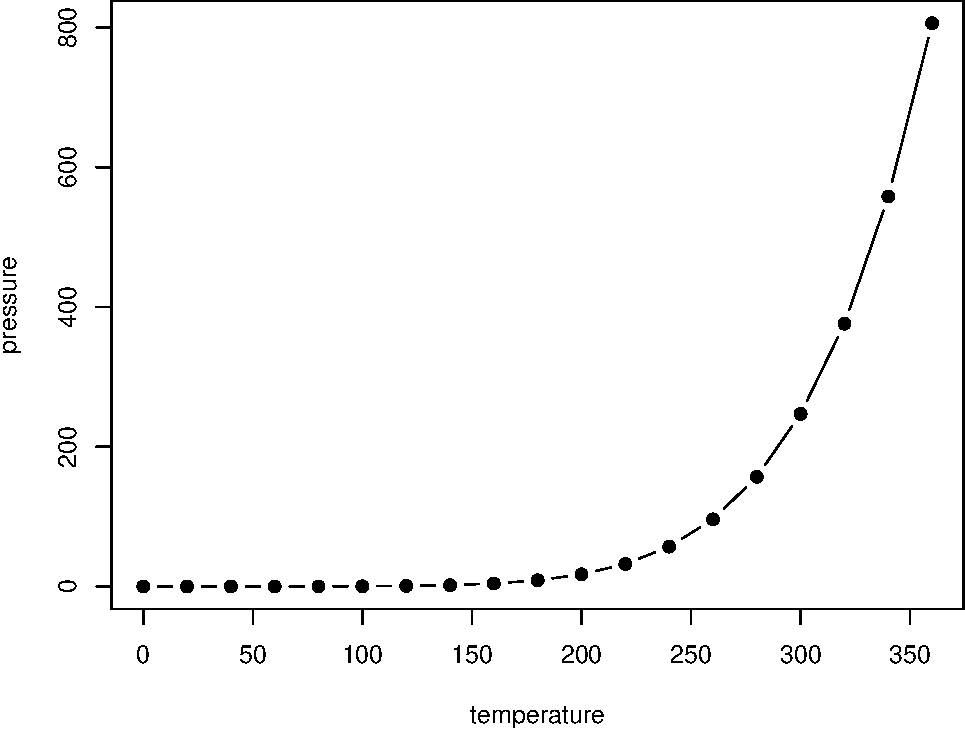
\includegraphics[width=0.8\linewidth]{badges4edu_files/figure-latex/nice-fig-1} 

}

\caption{Here is a nice figure!}\label{fig:nice-fig}
\end{figure}

Reference a figure by its code chunk label with the \texttt{fig:}
prefix, e.g., see Figure \ref{fig:nice-fig}. Similarly, you can
reference tables generated from \texttt{knitr::kable()}, e.g., see Table
\ref{tab:nice-tab}.

\begin{Shaded}
\begin{Highlighting}[]
\OperatorTok{>}\StringTok{ }\NormalTok{knitr}\OperatorTok{::}\KeywordTok{kable}\NormalTok{(}
\OperatorTok{+}\StringTok{   }\KeywordTok{head}\NormalTok{(iris, }\DecValTok{20}\NormalTok{), }\DataTypeTok{caption =} \StringTok{'Here is a nice table!'}\NormalTok{,}
\OperatorTok{+}\StringTok{   }\DataTypeTok{booktabs =} \OtherTok{TRUE}
\OperatorTok{+}\StringTok{ }\NormalTok{)}
\end{Highlighting}
\end{Shaded}

\begin{table}

\caption{\label{tab:nice-tab}Here is a nice table!}
\centering
\begin{tabular}[t]{rrrrl}
\toprule
Sepal.Length & Sepal.Width & Petal.Length & Petal.Width & Species\\
\midrule
5.1 & 3.5 & 1.4 & 0.2 & setosa\\
4.9 & 3.0 & 1.4 & 0.2 & setosa\\
4.7 & 3.2 & 1.3 & 0.2 & setosa\\
4.6 & 3.1 & 1.5 & 0.2 & setosa\\
5.0 & 3.6 & 1.4 & 0.2 & setosa\\
\addlinespace
5.4 & 3.9 & 1.7 & 0.4 & setosa\\
4.6 & 3.4 & 1.4 & 0.3 & setosa\\
5.0 & 3.4 & 1.5 & 0.2 & setosa\\
4.4 & 2.9 & 1.4 & 0.2 & setosa\\
4.9 & 3.1 & 1.5 & 0.1 & setosa\\
\addlinespace
5.4 & 3.7 & 1.5 & 0.2 & setosa\\
4.8 & 3.4 & 1.6 & 0.2 & setosa\\
4.8 & 3.0 & 1.4 & 0.1 & setosa\\
4.3 & 3.0 & 1.1 & 0.1 & setosa\\
5.8 & 4.0 & 1.2 & 0.2 & setosa\\
\addlinespace
5.7 & 4.4 & 1.5 & 0.4 & setosa\\
5.4 & 3.9 & 1.3 & 0.4 & setosa\\
5.1 & 3.5 & 1.4 & 0.3 & setosa\\
5.7 & 3.8 & 1.7 & 0.3 & setosa\\
5.1 & 3.8 & 1.5 & 0.3 & setosa\\
\bottomrule
\end{tabular}
\end{table}

You can write citations, too. For example, we are using the
\textbf{bookdown} package \citep{R-bookdown} in this sample book, which
was built on top of R Markdown and \textbf{knitr} \citep{xie2015}.

\section{My own (miscellanous) tests}\label{my-own-miscellanous-tests}

\subsection{Install stackr with
vignettes}\label{install-stackr-with-vignettes}

Building vignettes takes some time. So if you are in a hurry, than just
install stackr. You can still look at the vignettes in R help. The
difference is: With \texttt{build\_vignettes\ =\ TRUE} and then
\texttt{browseVignettes("stackr")} you can look at the vignettes in your
default browser. This is slightly more comfortable.

\begin{Shaded}
\begin{Highlighting}[]
\OperatorTok{>}\StringTok{ }\NormalTok{devtools}\OperatorTok{::}\KeywordTok{install_github}\NormalTok{(}\StringTok{"dgrtwo/stackr"}\NormalTok{, }\DataTypeTok{build_vignettes =} \OtherTok{TRUE}\NormalTok{)}
\OperatorTok{>}\StringTok{ }\KeywordTok{browseVignettes}\NormalTok{(}\StringTok{"stackr"}\NormalTok{)}
\end{Highlighting}
\end{Shaded}

\section{Load several packages at
once}\label{load-several-packages-at-once}

The following code is part of a debate at SO with different suggestions.
It seems to me, that all suggestions (utility packages, code examples)
has some disadvantages:

\begin{itemize}
\tightlist
\item
  \textbf{lapply:} For me the
  \href{https://stackoverflow.com/questions/8175912/load-multiple-packages-at-once}{best}
  approach -- it uses just \texttt{lapply}. I have changed
  \texttt{require} to \texttt{library} because of the arguments by
  \href{https://yihui.name/en/2014/07/library-vs-require/}{Yihui}. My
  lines now gives a error message and stops if one of the called
  packages is not installed.
\item
  \textbf{easypackages:} is not available on CRAN anymore, has very poor
  downloads.
\item
  \textbf{pacman:} a very sophisticated programm, but -- for me at least
  -- to complex and therefore to much overhead.
\item
  \textbf{installed.packages:}
  \href{https://gist.github.com/stevenworthington/3178163}{ipak.R} This
  loads \emph{and} installs missing packages. It is quite similar as
  \texttt{lappy}-version, but -- because of the if-condition -- more
  complex. Additionally it is checking which packages are installed:
\end{itemize}

\begin{quote}
``This can be slow when thousands of packages are installed, so do not
use this to find out if a named package is installed (use system.file or
find.package) nor to find out if a package is usable (call require and
check the return value) \ldots{}''
\end{quote}

So maybe the best would be to combine the \texttt{lapply} with the
\texttt{installled.packages} version. But insted to use
\texttt{installled.packages} I should use in the if-statement
\texttt{require}, check for the return value and -- if necessary -- to
install missing packages.

\begin{Shaded}
\begin{Highlighting}[]
\OperatorTok{>}\StringTok{ }\NormalTok{x <-}\StringTok{ }\KeywordTok{c}\NormalTok{(}\StringTok{"plyr"}\NormalTok{, }\StringTok{"psych"}\NormalTok{, }\StringTok{"tm"}\NormalTok{)}
\OperatorTok{>}\StringTok{ }\KeywordTok{lapply}\NormalTok{(x, library, }\DataTypeTok{character.only =} \OtherTok{TRUE}\NormalTok{)}
\end{Highlighting}
\end{Shaded}

\subsection{How many downloads of a defined
packages?}\label{how-many-downloads-of-a-defined-packages}

\begin{Shaded}
\begin{Highlighting}[]
\OperatorTok{>}\StringTok{ }\KeywordTok{library}\NormalTok{(dlstats)}
\OperatorTok{>}\StringTok{ }\NormalTok{y <-}\StringTok{ }\KeywordTok{cran_stats}\NormalTok{(}\StringTok{"learnr"}\NormalTok{)}
\OperatorTok{>}\StringTok{ }\KeywordTok{ggplot}\NormalTok{(y, }\KeywordTok{aes}\NormalTok{(start, downloads, }\DataTypeTok{group =}\NormalTok{ package, }\DataTypeTok{color =}\NormalTok{ package)) }\OperatorTok{+}
\OperatorTok{+}\StringTok{         }\KeywordTok{geom_line}\NormalTok{() }\OperatorTok{+}\StringTok{ }\KeywordTok{geom_point}\NormalTok{(}\KeywordTok{aes}\NormalTok{(}\DataTypeTok{shape =}\NormalTok{ package))}
\end{Highlighting}
\end{Shaded}

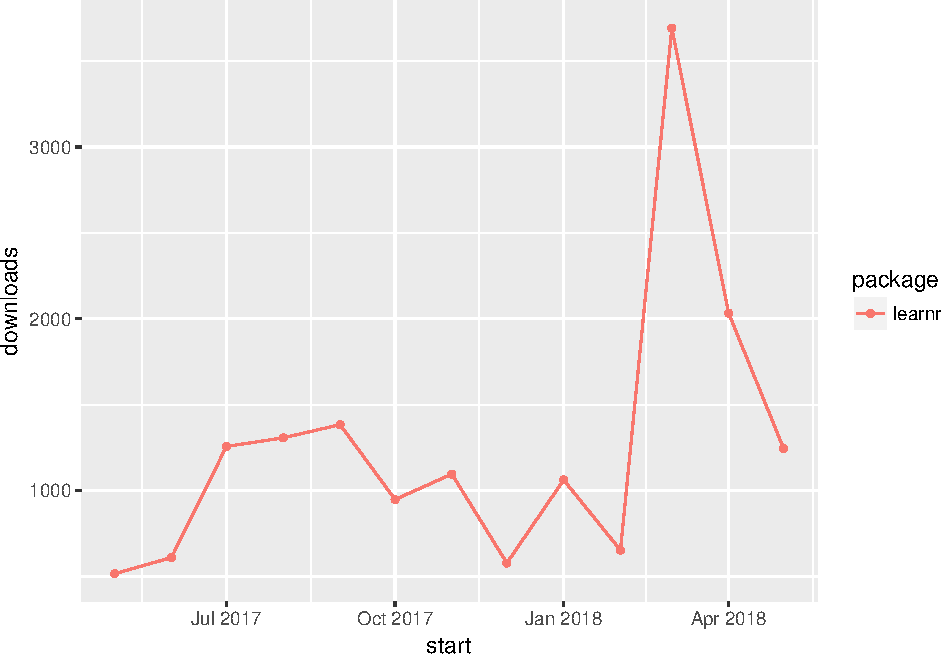
\includegraphics{badges4edu_files/figure-latex/download-stats-1.pdf}

\begin{Shaded}
\begin{Highlighting}[]
\OperatorTok{>}\StringTok{ }\CommentTok{# cranApp()}
\end{Highlighting}
\end{Shaded}

\section{Some data to remind}\label{some-data-to-remind}

\begin{enumerate}
\def\labelenumi{\arabic{enumi}.}
\tightlist
\item
  How to find answers tagged with \texttt{r} and not active since 6
  month:
  \href{https://stackoverflow.com/search?q=\%5Br\%5D+lastactive\%3A..6m+is\%3Aa}{Search}
\end{enumerate}

\begin{enumerate}
\def\labelenumi{\arabic{enumi}.}
\setcounter{enumi}{2}
\tightlist
\item
  What kind of actions are are allowed with \texttt{combine\_url}?
\end{enumerate}

I have added \texttt{timeline} to the list!

\subsection{Some experiments}\label{some-experiments}

\bibliography{book.bib,packages.bib}


\end{document}
